\chapter{Tools}
\label{chapter:tools}

The next sections present the most important programming tools used \ignore{in the implementation of} to build the conversational agent. The first two sections describe tools that are part of the ontological approach to the implementation of the program. The next ones discuss tools used in both the initial method and the answer sentence selection approach.

\section[DBpedia]{DBpedia}
\label{sec:dbpedia}

DBpedia\footnote{\href{dbpedia.org}{DBpedia}, \url{dbpedia.org}} is a project that aims to convert content extracted from Wikipedia into a structured dataset, that is subsequently made available on the World Wide Web. The final purpose of this project is to provide an interface so that the users can query Wikipedia in a structured manner using Semantic Web techniques. The structured information is published using the RDF\footnote{\href{http://www.w3.org/RDF/}{Resource Description Framework}, \url{http://www.w3.org/RDF/}} specifications. In addition, DBpedia links its dataset with other published open datasets, in total reaching 2 billion RDF triples (in 2007) \cite{Auer2007}.

The DBpedia datasets can be accessed in three ways:
\begin{itemize}
  \item through the Linked Data interface, where the DBpedia resources (published as RDF data) can be accessed using URIs.
  \item using the SPARQL Endpoint that supports specific SPARQL queries.
  \item downloading RDF dumps containing larger parts of the DBpedia dataset.
\end{itemize}

The important aspect of DBpedia for building our \ignore{ok to say our?} conversational agent is that DBpedia has a separate, independent {\em Persons} dataset that has more than half a million RDF triples containing information (extracted from Wikipedia articles written in English) for around 760,000 people, as of 2012 \cite{Lehmann2012}.

\section[ChatScript]{ChatScript}
\label{sec:chatscript}

ChatScript\footnote{\href{http://chatscript.sourceforge.net/}{ChatScript}, \url{http://chatscript.sourceforge.net/}} is an engine for building conversational agents. ChatScript is a rule-based system relying on its own scripting language (similar to AIML\footnote{\href{http://www.alicebot.org/aiml.html}{AIML: Artificial Intelligence Markup Language}, \url{http://www.alicebot.org/aiml.html}}) to model the conversational behavior of an agent. Its purpose is to "pattern-match on general meaning" by using "sets of words and canonical representation." \cite{Wilcox2011}

A chat-bot is modeled through a set of script files that contain rules. A rule is formed from a pattern and a response. The response represents the output that a ChatScript bot will provide if the input matches the pattern. Two ChatScript rules are presented in \autoref{chatscript-listing}.  The elements in the parentheses constitute the pattern and the sentence after the pattern represents the answer returned if the user input matches the pattern. The $ * $ (star) symbol is a wildcard that can match none, one or more words.

\begin{lstlisting}[float=htb,numbers=none, caption=ChatScript rules example, label=chatscript-listing]
u: ( Where * you * born ) In the capital.
u: ( When * born ) This century.
\end{lstlisting}

\section[WordNet]{WordNet}
\label{sec:wordnet}

WordNet\footnote{\href{http://wordnet.princeton.edu}{Princeton University "About WordNet." WordNet. Princeton University. 2010.}, \url{http://wordnet.princeton.edu}} is an online lexical reference database \cite{Miller1990,Miller1995} containing: words, lexical relations and sematic relations.

{\em Word.} A word is defined as a pair ({\em f}, {\em m}) between a form {\em f} (the string representation of the word) and a meaning {\em m}. If a word has more than one meaning (it is polysemous), WordNet differentiates between the meanings and keeps a pair ({\em f}, {\em m}) for each meaning. The polysemy of a word can be extended to its part of speech, i.e. a word can have different meanings depending on its part of speech; e.g. {\em die} can be a polysemous noun meaning either {\em dice} or is "a device used for shaping metal", or a verb meaning {\em decease}. In the WordNet database only "open-class words" are present. The database includes about 155,000 nouns, verbs, adverbs and adjectives \cite{Fellbaum1998}.

{\em Synonym set.} The words are grouped into synonym sets, also known as {\em synsets}, which are the core element in WordNet. A synset is used to represent the meaning (or sense) of a word \cite{Miller1995}.

{\em Lexical relations.} A lexical relation between two words is a relation between the form of the words. For example, synonymy and antonymy is stored in the database as a lexical relation \cite{Miller1990}.

{\em Semantic relations.} A semantic relation is a relation between word meanings and is stored in the WordNet database as a pointer between synsets. The semantic relations between the synsets are useful to model concepts like: hyponymy, hypernymy, meronymy etc.

\subsection{MIT Java WordNet Interface}
\label{sub-sec:wordnet-jwi}

The Java WordNet Interface (JWI) is an Application Programming Interface (API) written for the Java programming language that is used to access and query the WordNet database files. JWI features calls to retrieve index words and synsets and calls that allow following lexical and semantic pointers \cite{Finlayson2011}. Mainly, it can be used to access synonyms, antonyms and hypernyms/hyponyms of a given word. Three most important advantages to use JWI as presented in \cite{Finlayson2013} are:
\begin{itemize}
  \item JWI provides both file-based and in-memory dictionary implementations, allowing you to trade off speed and memory consumption
  \item JWI sets no limit on the number of dictionaries that may be instantiated in each JVM
  \item JWI is high-performance, with top-ranked speeds on various retrieval metrics and in-memory dictionary load time
\end{itemize}
It can be seen in the benchmarks from \cite{Finlayson2013} that JWI is one of the fastest libraries for WordNet. Average access time for retrieval of an entry and for iterating through entries in the database are shown in \autoref{table:wordnet-access-time}.

\begin{table}[htb]
  \centering
  \begin{tabular}{lcc}
    Object & Retrieval time ($\mu$s) & Iteration time ($\mu$s) \\
    \hline
    Index Word & 12.3 & 296 \\
    Synset & 7.1 & 798\\
    Word-by-Sense-Key & 17.2 & 141\\
    Exception Entry & 16.1 & 4 \\
    Synsets by Index Word & - & 1.8s \\
  \end{tabular}
  \caption{Average time of access of WordNet database}
  \label{table:wordnet-access-time}
\end{table}

\section{Apache Lucene}
\label{sec:lucene}

Apache Lucene\footnote{\href{https://lucene.apache.org/core/}{Apache Lucene Core}, \url{https://lucene.apache.org/core/}} is a text-search library written in Java. It provides an API for performing common search tasks like text indexing, querying, highlighting results and others \cite{Biaecki2012}. Lucene achieves high performance due to the inverted index \cite{VanRijsbergen1979} approach. In addition, the search speed can be increased by placing the text in memory, using the RAMDirectory class.

Lucene's three main features, presented below, are: analysis of incoming content and queries, indexing and storage and searching \cite{Biaecki2012}.

{\em Language Analysis}. The texts to be searched and the queries are stored internally in a modified form for faster access. The transformations made are: character filtering, tokenization, stemming, lemmatization, stopwords removal and others.

{\em Indexing and storage}. Lucene supports inverted indexes on more than one field per document, useful for annotating the text with different information (e.g. ISBN). All this data can be stored on a persistent device (for large sets of documents) or, as previously stated, in the RAM memory for faster access (for reduced size documents). In addition, Lucene can be configured to use different kinds of query scoring, based on total word frequency, unique word count and total document frequency of all words \cite{Biaecki2012}.

{\em Searching}. The implementation of Lucene's querying supports several types of searching mechanisms, like: wildcards, fuzzy search, proximity search, binary operators and others \cite{Biaecki2012}. Querying can be optimized by providing a number of top matches after which the search stops.

\section{Stanford CoreNLP}
\label{sec:corenlp}

Stanford CoreNLP is one of the most exhaustive tools for natural language analysis. It is an open source project written in Java and has a comprehensive API that is easy to use. Architecturally, Stanford CoreNLP is a pipeline that annotates the input text with relevant information, like the part of speech of the words. It also generates graph-like structures containing links between words, representing relations like: syntactic dependencies and co-references. The execution flow of the annotator is represented in \autoref{fig:corenlp-pipeline}.

The provided annotators that can be included in the processing are: "tokenize", "cleanxml", "ssplit", "truecase", "pos", "lemma", "gender", "ner", "regexner", "parse", "sentiment" and "dcoref". Most of the annotators are built as separate modules that are integrated afterwards in the core. Some of these main modules are presented in the following sections.

\begin{figure}[htb]
  \centering
  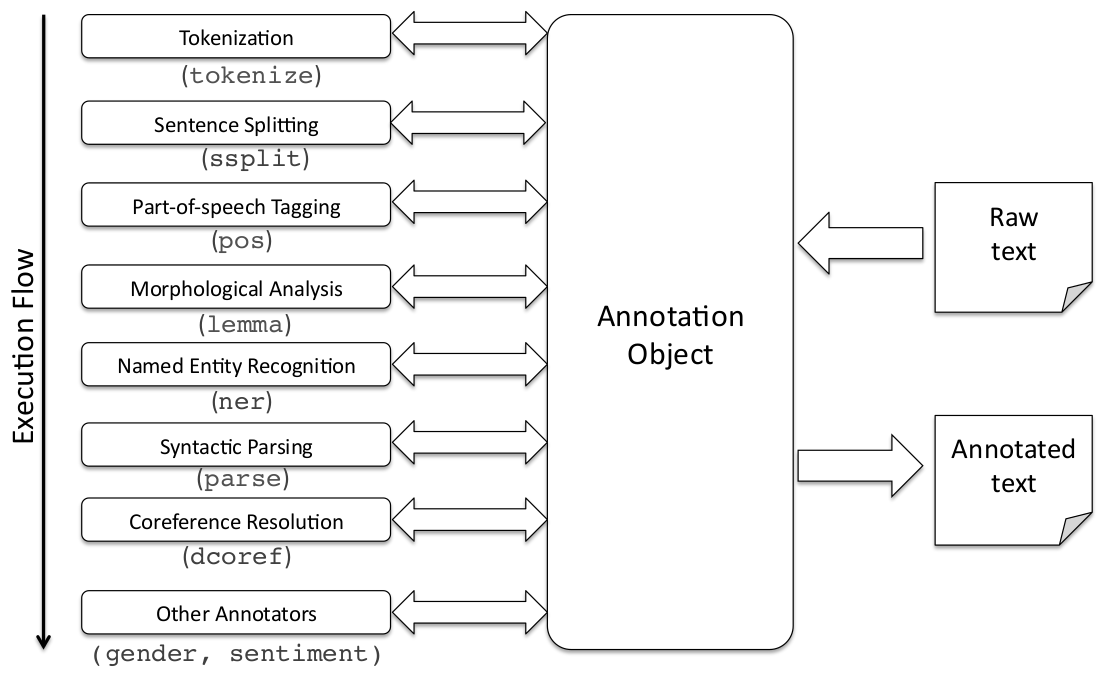
\includegraphics[width=\textwidth]{src/img/corenlp-pipeline.png}
  \caption[Stanford CoreNLP execution pipeline]{Stanford CoreNLP execution pipeline \cite{Manning2014}}
  \label{fig:corenlp-pipeline}
\end{figure}

\subsection{Stanford Tokenizer}
\label{sub-sec:stanford-tokenizer}

Although the tokenizer is not an independent part of the Stanford NLP project, it appears in multiple modules of the project. The role of the tokenizer is to split the raw text into a sequence of individual tokens \cite{Manning2014}. The tokenizer uses Penn Treebank style tokenization\footnote{\href{https://www.cis.upenn.edu/~treebank/tokenization.html}{Penn Treebank Tokenization Specifications}, \url{https://www.cis.upenn.edu/~treebank/tokenization.html}}. The functionality of the tokenizer is implemented in the {\em PTBTokenizer} Java class.

During the tokenization process, besides the actual list of tokens, the {\em PTBTokenizer} also generates a text annotation for each token in order to retrieve the original form of the text when needed. This is mostly useful when the lemmatization process, described below, is applied to the text.

Another use for the tokenizer is to accomplish sentence splitting (added with the "ssplit" annotator option as mentioned before). This is done by tokenization after one of the sentence-ending characters (\textbf{.}, \textbf{!} and \textbf{?}) if they are not grouped with other characters into a token (such as for an abbreviation or number) \cite{StanfordTokenizer}.

After the tokenization has been performed, the individual words can be lemmatized (using the "lemma" annotator option), meaning that a word is annotated with its dictionary form (or base form). For example: {\em has}, {\em had} and {\em having} become {\em have}; {\em children}, {\em child's} and {\em children's} become {\em child}.

\subsection{Stanford Log-linear Part-Of-Speech Tagger}
\label{sub-sec:stanford-pos}

The purpose of the Part-Of-Speech (POS) tagger is to label words with their corresponding POS tag, using a maximum entropy POS tagger \cite{Manning2014}. The English POS tagger uses the Penn Treebank tagset described in \cite{Marcus1993}. This type of tagging is particularly useful for syntactic analysis in NLP applications, for example it is important to determine a word's part of speech when finding the appropriate synonym for the word if the word is polysemous.

The POS tagger uses a cyclic dependency network model trained using lexical features of words extracted from the Penn Treebank dataset. The network is then used as a classifier fed with the given text as input. The architecture of the dependency network used for feature-rich POS tagging is described in depth in \cite{Toutanova2003}.

\subsection{Stanford Named Entity Recognizer}
\label{sub-sec:stanford-ner}

The Stanford Named Entity Recognizer (NER) is an annotation tool that labels words (or sequence of words) that are likely to stand for names of things (like people and places). Stanford NER uses a statistical model trained on a collection of Reuters articles annotated with four entity types: person (PER), location (LOC), organization (ORG), and miscellaneous (MISC) \cite{Finkel2005}. The Stanford NER dataset contains statically assigned types for a set of entities, but it can also infer the type from the context, as seen in \autoref{table:stanford-ner}. \autoref{table:stanford-ner} shows that {\em Bucharest} is a known entity with its type previously assigned as opposed to {\em Ploiești} which is wrongly considered a person in the sentence {\em "I like Ploiești"}. Despite this fact, the NER successfully identifies {\em Ploiești} as a location in the {\em "I live in Ploiești"} sentence.

Stanford NER is useful for the Stanford Co-Reference System, described in \autoref{sub-sec:stanford-dcoref}, where a relation needs to be established between a pronoun (her, his, it etc.) and a name of a person.

\begin{table}[htb, width=\textwidth]
  \centering
  \begin{tabular}{lcc}
    Sentence & Token & NER \\
    \hline
    {\em I like Bucharest} & Bucharest & Location \\
    {\em I live in Bucharest} & Bucharest & Location \\
    {\em I like Ploiești} & Ploiești & Person \\
    {\em I live in Ploiești} & Ploiești & Location \\
  \end{tabular}
  \caption{Inference of types using the Named Entity Recognizer}
  \label{table:stanford-ner}
\end{table}

\subsection{Stanford Deterministic Coreference Resolution System}
\label{sub-sec:stanford-dcoref}

Stanford's Coreference Resolution System implements mention detection and both pronominal and nominal co-reference resolution \cite{Manning2014}. This tool is used to link pronouns to the entities they refer to. In order to achieve that, the architecture of the system applies several deterministic co-reference models, one after the other. The first, and most important step of this algorithm is the {\em mention detection}, where the nominal and pronominal mentions are identified using an algorithm that selects all noun phrases, pronouns and named entity mentions. After that, the co-reference models are applied from highest to lowest precision. All the steps of the algorithm are described in \cite{Lee2013}.

An example of this system's functionality is presented in \autoref{fig:dcoref}, where the pronoun {\em he} is linked to the word {\em Lennon}, the name of the person the pronoun refers to.

\begin{figure}[htb]
  \centering
  \captionsetup{justification=centering}
  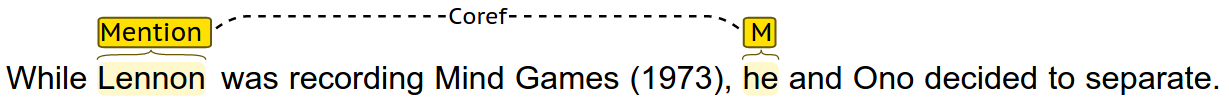
\includegraphics[width=\textwidth]{src/img/dcoref.png}
  \caption[A co-reference example]{A co-reference example where the mention of the pronoun {\em he} is connected by the {\em coref}-type relation with the mention of the enitity {\em Lennon}}
  \label{fig:dcoref}
\end{figure}

\pagebreak

\ignore{
\subsection{Stanford Parser}
\label{sub-sec:stanford-parser}
}
